% !TeX encoding = UTF-8

%% ------------------------------------------------------------------------
%% Copyright (C) 2021 SJTUG
%% 
%% SJTUBeamer Example Document by SJTUG
%% 
%% SJTUBeamer Example Document is licensed under a
%% Creative Commons Attribution-NonCommercial-ShareAlike 4.0 International License.
%% 
%% You should have received a copy of the license along with this
%% work. If not, see <http://creativecommons.org/licenses/by-nc-sa/4.0/>.
%% -----------------------------------------------------------------------

\documentclass[xcolor=table,dvipsnames,svgnames,aspectratio=169]{ctexbeamer}
% 可以通过 fontset=macnew / fontset=ubuntu / fontset=windows 选项切换字体集

\usepackage{tikz}
\usepackage[normalem]{ulem}
\usetikzlibrary{arrows}
\usepackage{amsmath}
\usepackage{mflogo}
\usepackage{graphicx}
\usepackage{xspace}
\usepackage{amsmath}
\usepackage{unicode-math}
\usepackage{ccicons}
\usepackage{hologo}
\usepackage{colortbl}
\usepackage{shapepar}
\usepackage{hyperxmp}
\usepackage{booktabs}
\usepackage{qrcode}
\usepackage{listings}
\usepackage{tipa}
\usepackage{multicol}
\usepackage{datetime2}
\usepackage{fontawesome5}
\usepackage{hyperref}
\usepackage[backend=biber,style=gb7714-2015]{biblatex}

\addbibresource{proposal.bib}
\setbeamertemplate{bibliography item}[text]

\graphicspath{{figures/}}

\hypersetup{
  pdfsubject = {PhD-ResearchProposal},
  pdfauthor = {Pedro Hernández Rubio},
  pdfcopyright = {Licensed under CC-BY-SA 4.0. Some rights reserved.},
  pdflicenseurl = {http://creativecommons.org/licenses/by-sa/4.0/},
  unicode            = true,
  psdextra           = true,
  pdfdisplaydoctitle = true
}

\pdfstringdefDisableCommands{
  \let\\\relax
  \let\quad\relax
  \let\hspace\@gobble
}

\renewcommand{\TeX}{\hologo{TeX}}
\renewcommand{\LaTeX}{\hologo{LaTeX}}
\newcommand{\BibTeX}{\hologo{BibTeX}}
\newcommand{\XeTeX}{\hologo{XeTeX}}
\newcommand{\pdfTeX}{\hologo{pdfTeX}}
\newcommand{\LuaTeX}{\hologo{LuaTeX}}
\renewcommand{\CTeX}{C\TeX}
\newcommand{\MiKTeX}{\hologo{MiKTeX}}
\newcommand{\MacTeX}{Mac\hologo{TeX}}
\newcommand{\beamer}{\textsc{beamer}}
\newcommand{\XeLaTeX}{\hologo{Xe}\kern-.13em\LaTeX{}}
\newcommand{\pdfLaTeX}{pdf\LaTeX{}}
\newcommand{\LuaLaTeX}{Lua\LaTeX{}}

\def\TeXLive{\TeX{} Live\xspace}
\let\TL=\TeXLive
\newcommand{\SJTUThesis}{\textsc{SJTUThesis}\xspace}
\newcommand{\SJTUBeamer}{\textsc{SJTUBeamer}\xspace}
\newcommand{\SJTUThesisVersion}{1.0.0rc7}
\newcommand{\SJTUThesisDate}{2020/7/31}

\newcommand\link[1]{\href{#1}{\faLink}}
\newcommand\pkg[1]{\texttt{#1}}

\def\cmd#1{\texttt{\color{DarkBlue}\footnotesize $\backslash$#1}}
\def\env#1{\texttt{\color{DarkBlue}\footnotesize #1}}
\def\cmdxmp#1#2#3{\small{\texttt{\color{DarkBlue}$\backslash$#1}\{#2\}\hspace{1em}\\ $\Rightarrow$\hspace{1em} {#3}\par\vskip1em}}

\lstset{
  language=[LaTeX]TeX,
  basicstyle=\ttfamily\footnotesize,
  tabsize=2,
  keywordstyle=\bfseries\ttfamily\color{cprimary},
  commentstyle=\sl\ttfamily\color[RGB]{100,100,100},
  stringstyle=\ttfamily\color[RGB]{50,50,50},
  extendedchars=true,
  breaklines=true,
}

\lstdefinestyle{style@inline}{
  basicstyle   = \ttfamily,
  keepspaces   = true
}
\lstMakeShortInline[style=style@inline]|

\usetheme[maxplus]{sjtubeamer}
% 使用 maxplus/max/min 切换标题页样式
% 使用 red/blue 切换主色调
% 使用 light/dark 切换亮/暗色模式
% 使用外样式关键词以获得不同的边栏样式
%   miniframes infolines  sidebar* 
%   default    smoothbars split	 
%   shadow     tree       smoothtree
% *siderbar 推荐与 max 一起使用。

% \tikzexternalize[prefix=cache/]
% 如果您需要缓存 tikz 图像,请取消注释上一行,并在编译选项中添加 -shell-escape。

\author{Hugo Vanhille, Pedro Hernández Rubio}
\institute[SEIEE]{Department of Automation}
\date{\the\year 年 \the\month 月}
\subject{ECE6903J - Distributed Machine Learning Systems}
\title{Blockchain-based incentive mechanisms in Federated Learning}
\title[Research project proposal (Group 4)] % 页脚显示标题
{\textbf{Blockchain-based incentive mechanisms in Federated Learning}} % 首页标题

\subtitle{ECE6903J - Distributed Machine Learning Systems (Group 4)}
%\subtitle{Evaluation of blockchain technology in student mobility administration process}

\begin{document}

% 使用节目录
\AtBeginSection[]{
  \begin{frame}
    % \tableofcontents[currentsection]           % 传统节目录             
    \sectionpage                   % 节页
  \end{frame}
}

% 使用小节目录
\AtBeginSubsection[]{                  % 在每小节开始
  \begin{frame}
    % \tableofcontents[currentsection,currentsubsection]             % 传统小节目录             
    \subsectionpage                % 小节页
  \end{frame}
}

\maketitle

\begin{frame}{目录}
\begin{multicols}{2}
  \tableofcontents
  \end{multicols}
\end{frame}

% !TeX encoding = UTF-8
% !TeX root = ../main.tex

%% ------------------------------------------------------------------------
%% Copyright (C) 2021 SJTUG
%% 
%% SJTUBeamer Example Document by SJTUG
%% 
%% SJTUBeamer Example Document is licensed under a
%% Creative Commons Attribution-NonCommercial-ShareAlike 4.0 International License.
%% 
%% You should have received a copy of the license along with this
%% work. If not, see <http://creativecommons.org/licenses/by-nc-sa/4.0/>.
%% -----------------------------------------------------------------------

\section{Background}

\subsection{Motivation}

\begin{frame}{Motivation}
	\begin{block}{Goal}
        Applying ML to systems (blockchain-based models)
      \end{block}
  \begin{itemize}
    \item Research line mainly targeted to \alert{blockchain technology} (its application to systems)
    \item Research group in Department of Automation (PhD supervisors) has been recently working in blockchain-based models applied to \alert{trust management systems}
	\item Specifically, applied to data-aggregation systems in the Internet of Things (IoT) field \alert{crowdsensing}
	\item Could similar approach be applied for \alert{Federated Learning}?
%    \item My PhD thesis could use some of the model simulation techniques (stochastic processes) used in this research paper experimentation
%    \item And of course, it is related to a emerging subfield that could greatly contribute to the development of the Internet of Things (IoT)
  \end{itemize}
\end{frame}

\subsection{Federated Learning}

\begin{frame}{Federated Learning: definition}
  \begin{itemize}
  \item \textbf{Crowdsensing:} emerging paradigm of data aggregation\cite{paper1}, having a key role in data-driven applications. Specially used for getting large ammounts of IoT sensing data, by using the individual intelligent sensing devices.
  \item \textbf{Benefit:} improved data collection efficiency and reduced costs effectively\cite{paper2}
  \end{itemize}
  \begin{figure}[h]
        \centering
        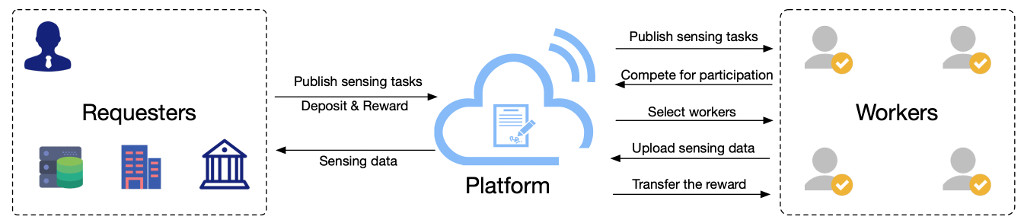
\includegraphics[width=.8\textwidth]{201909-wei-figure1.jpg}
      \end{figure}
\end{frame}

\begin{frame}{Federated Learning: issues}
  		\begin{enumerate}
   			\item Managed and maintained \alert{centralized platforms} suffer from the single point of failure
   				\begin{itemize}
   					\item \textbf{Proposal: } decentralized architecture (blockchain technology) that lacks a single point of failure, and enhances privacy with asymmetric encryption and digital signature technology
   				\end{itemize}
    		\item Encouraging workers by offering appropiate \alert{incentive mechanisms} (monetary usually) \rightarrow  \underline{auction theory} guarantees benefits for both requesters and workers\cite{paper15} but only provide short-term incentives
    			\begin{itemize}
   					\item \textbf{Proposal:} hybrid incentive mechanism, adopting \underline{mechanism design theory}, considering three factors:
   					\begin{itemize}
   					\item Monetary reward
   					\item Reputation evaluation
   					\item Data quality
   					\end{itemize}
   				\end{itemize}
  		\end{enumerate}
\end{frame}

\subsection{Blockchain technology}

\begin{frame}{Blockchain background}
  \alert{Distributed ledger containing a time-stamped series of immutable blockchains, trustless, decentralized, proof-tampering and full traceability}
  \begin{itemize}
    \item Research approaches on blockchain-based Federated Learning:
          \begin{itemize}
            \item Evaluating time consumption and task cost of applying a blockchain-based system\cite{paper33}
            \item Blockchain-based crowdsensing quality control model\cite{paper34}
            \item Considering privacy issues\cite{paper35}
            \item Handling location privacy protection\cite{paper37} (confusion mechanism)
          \end{itemize}
  \end{itemize}
\end{frame}
% !TeX encoding = UTF-8
% !TeX root = ../main.tex

%% ------------------------------------------------------------------------
%% Copyright (C) 2021 SJTUG
%% 
%% SJTUBeamer Example Document by SJTUG
%% 
%% SJTUBeamer Example Document is licensed under a
%% Creative Commons Attribution-NonCommercial-ShareAlike 4.0 International License.
%% 
%% You should have received a copy of the license along with this
%% work. If not, see <http://creativecommons.org/licenses/by-nc-sa/4.0/>.
%% -----------------------------------------------------------------------

\section{Research problems}

\subsection{The incentive mechanism}

\begin{frame}{Application to Federated Learning}
  \begin{itemize}
    \item Main types of incentive mechanisms:
          \begin{enumerate}
            \item \alert{Monetary-based}: distributing rewards. And two subtypes can be considered\cite{paper16}:
            	\begin{itemize}
            	\item \alert{price-decision-first} (auction theory) design optimal mechanism benefiting both requesters adn workers
            	\item \alert{upload-decision-first}: distributing rewards base on the uploaded data (quality)
          		\end{itemize}
            \item \alert{Reputation-based}: reputation framework for worker selection (algorithms)
          \end{enumerate}
    \item \textbf{Limitations}
    	\begin{enumerate}
            \item Relies on a central platform, vulnerable to target attacks
            \item Single-attribute incentive mechanisms (multifactor incentive needed)
          \end{enumerate}
     Some previous hybrid incentive mechanisms\cite{paper52} suffer of usability problems because the difficulty of hybrid data management
  \end{itemize}
\end{frame}

\subsection{Benefits and limitations}

\begin{frame}{Benefits}
	A consortium blockchain-based incentive model for Federated Learning system is
proposed
  \begin{itemize}
  \item \textbf{Benefits of consortium blockchain technology:} 
  	\begin{itemize}
  		\item resistant to the single point of failure (system security)
  		\item cooperative management (by requesters) reduces cost and enhances the flexibility of the system (selection criteria)
  	\end{itemize}
  \item \textbf{Benefits of hybrid incentive mechanism:}
  	\begin{itemize}
  		\item encourages workers to contribute valuable data (and penalizes malicious ones)
  		\item ensures favorables short-term and long-term incentives for workers
  	\end{itemize}
  \end{itemize}
\end{frame}

\begin{frame}{Limitations}
	Further research:
  \begin{enumerate}
  \item Dynamic situation where evaluations attributes are changing
  \item Optimization of consensus protocol (better performance)
  \item Further protection of worker privacy
  \end{enumerate}
  \begin{block}{Possible solutions}
  Application of ML techniques to blockchain-based system
  \end{block}
\end{frame}
%% !TeX encoding = UTF-8
% !TeX root = ../main.tex

%% ------------------------------------------------------------------------
%% Copyright (C) 2021 SJTUG
%% 
%% SJTUBeamer Example Document by SJTUG
%% 
%% SJTUBeamer Example Document is licensed under a
%% Creative Commons Attribution-NonCommercial-ShareAlike 4.0 International License.
%% 
%% You should have received a copy of the license along with this
%% work. If not, see <http://creativecommons.org/licenses/by-nc-sa/4.0/>.
%% -----------------------------------------------------------------------

\section{System architecture}

\subsection{Software application}

\begin{frame}{System architecture}
	\begin{figure}[h]
        \centering
        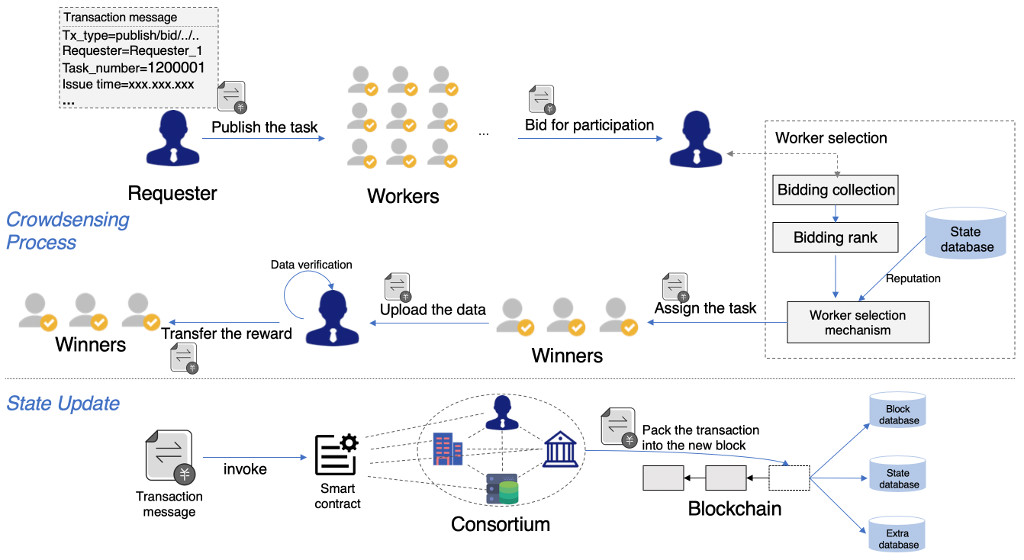
\includegraphics[width=.7\textwidth]{201909-wei-figure2.jpg}
      \end{figure}
\end{frame}

%\begin{frame}{Blockchain application}
%\begin{columns}[T,onlytextwidth]
%    \column{0.7\textwidth}
%	\begin{center}
%		\includegraphics[height=.8\textheight]{eductx.pdf}\hfill
%	\end{center}
%	\column{0.3\textwidth}
%%	\metroset{block=fill}
%      \begin{exampleblock}{Platform}
%        Ethereum
%      \end{exampleblock}
%      \begin{exampleblock}{NF tokens}
%        University credits
%      \end{exampleblock}
%      \begin{exampleblock}{Consensus}
%        Proof-of-stake
%      \end{exampleblock}
%      \begin{exampleblock}{Scope}
%        Public
%      \end{exampleblock}
%      \begin{exampleblock}{Licence}
%        Open source
%      \end{exampleblock}
%\end{columns}
%\end{frame}

%\begin{frame}{Blockchain application}
%  \begin{columns}[c]
%    \begin{column}{.45\textwidth}
%      \begin{itemize}
%        \item Platform
%              \begin{itemize}
%                \item Ethereum
%                \item Hyperledger
%              \end{itemize}
%        \item NF tokens: exchange students
%        \item Consensus: proof-of-stake
%        \item Scope: public
%		\item License: open source
%      \end{itemize}
%    \end{column}
%    \begin{column}{.45\textwidth}
%      \includegraphics[width=\textwidth]{eductx.pdf}
%    \end{column}
%  \end{columns}
%\end{frame}

\begin{frame}{System flow}
  \begin{itemize}
    \item \textbf{System initialization}: configuration and identity authentication mechanisms
    \item \textbf{Task process}: Specific steps of crowdsensing
          \begin{itemize}
            \item Step 1: \alert{Task publishing} (invoking the smart contract to update the task state)
            \item Step 2: \alert{Worker selection} (workers submit the bidding price and workers select appropiate workers)
            \item Step 3: \alert{Data uploading} (selected workers perform the task and upload data)
            \item Step 4: \alert{Reward assignment and data evaluation} (requester distribute rewards and evaluate data quality)
          \end{itemize}
     \item \textbf{System synchronization}: state update about tasks and workers (validating transactions into new blocks)
  \end{itemize}
\end{frame}

% !TeX encoding = UTF-8
% !TeX root = ../main.tex

%% ------------------------------------------------------------------------
%% Copyright (C) 2021 SJTUG
%% 
%% SJTUBeamer Example Document by SJTUG
%% 
%% SJTUBeamer Example Document is licensed under a
%% Creative Commons Attribution-NonCommercial-ShareAlike 4.0 International License.
%% 
%% You should have received a copy of the license along with this
%% work. If not, see <http://creativecommons.org/licenses/by-nc-sa/4.0/>.
%% -----------------------------------------------------------------------

\section{Related work}

\subsection{Blockchain-based Federated Learning}

\begin{frame}{Blockchain-based Federated Learning}
     Some previous hybrid incentive mechanisms\cite{paper52} suffer of usability problems because the difficulty of hybrid data management
\end{frame}

\begin{frame}
Advances and Open Problems in Federated Learning\cite{1912.04977}


This paper describes the defining characteristics and challenges of the federated learning setting.It highlights important practical constraints and considerations, and then enumerates a range of valuable
research directions. The goals of this paper are to highlight research problems that are of significant theoretical and practical interest, and to encourage research on problems that could have significant real-world impact
\end{frame}

\begin{frame}
Generative models for effective ML in  private, decentralized datasets\cite{1911.06679}


This document focuses on three main topics : 


-Identifying key challenges in implementing end-to-end workflows with non-inspectable data


-Proposing a methodology that allows ‘auxiliary’ generative models to resolve these challenges


-Demonstrating how privacy preserving federated generative models can be trained to high enough fidelity to discover introduced data errors matching
those encountered in real world scenarios
\end{frame}

\begin{frame}
Blockchain-based Federated Learning: A Comprehensive Survey\cite{Comprehensive_survey}


This paper conducts a comprehensive survey of the literature on blockchained FL (BCFL). First, it investigates how blockchain can be applied to federal learning from the perspective of system composition. Then, it analyzes the concrete functions of BCFL from the perspective of mechanism design and illustrate what problems blockchain addresses specifically for FL. Finally, it discusses some challenges and future research directions.
\end{frame}

\begin{frame}
Federated Learning Meets Blockchain in Edge Computing: Opportunities and Challenges\cite{nguyen_federated_2021}


This article presents an overview of the fundamental concepts and explores the opportunities of FL chain in mobile-edge computing networks in relation with his main issues in FL chain design such as communication cost, resource allocation, incentive mechanism, security and privacy protection. The key solutions and the lessons learned along with the outlooks are also discussed. Then, it investigates the applications of FL chain in popular Mobile-edge computing domains.
\end{frame}
\subsection{Incentive mechanisms applied to Federated Learning}

\begin{frame}{Incentive mechanisms applied to Federated Learning}
     Some previous hybrid incentive mechanisms\cite{paper52} suffer of usability problems because the difficulty of hybrid data management
\end{frame}

% !TeX encoding = UTF-8
% !TeX root = ../main.tex

%% ------------------------------------------------------------------------
%% Copyright (C) 2021 SJTUG
%% 
%% SJTUBeamer Example Document by SJTUG
%% 
%% SJTUBeamer Example Document is licensed under a
%% Creative Commons Attribution-NonCommercial-ShareAlike 4.0 International License.
%% 
%% You should have received a copy of the license along with this
%% work. If not, see <http://creativecommons.org/licenses/by-nc-sa/4.0/>.
%% -----------------------------------------------------------------------

\section{Planned solution}

\subsection{Mechanism design: multifactor}

\begin{frame}{Mechanism design: ML application?}
  \begin{itemize}
    \item Based on three parameters:
          \begin{enumerate}
            \item \alert{Workers' bidding}
            \item \alert{Reputation}
            \item \alert{Recent data quality estimation}
          \end{enumerate}
    \item Analytic Hierarchy Process (AHP) framework \rightarrow (top-down)
    	\begin{enumerate}
            \item \alert{Objective level}: winning workers
            \item \alert{Criteria level}: parameters criteria
            \item \alert{Alternative level}: workers available
          \end{enumerate}
    \end{itemize}
    \begin{exampleblock}{Multifactor worker evaluation approach (example)}
    	\begin{equation*}
      	\theta_{i}=\omega_{1} B_{i}+\omega_{2} R_{i}+\omega_{3} Q_{i} \quad\quad \text { where } \omega_{i} \geq 0 \text { and } \sum_{\omega_{i}=1}^{3} \omega_{i}=1	
    	\end{equation*}
  \end{exampleblock}
\end{frame}

\subsection{Mechanism design: issues}

\begin{frame}{Mechanism design: issues}
  		\begin{enumerate}
   			\item \textbf{How to select appropriate workers?}
   				\begin{itemize}
   					\item \textbf{Proposal: } decentralized architecture (blockchain technology) that lacks a single point of failure, and enhances privacy with asymmetric encryption and digital signature technology
   				\end{itemize}
    		\item \textbf{How to distribute the rewards to the workers?}
  		\end{enumerate}
  		With the help of \alert{mechanism design theory}\cite{article56} two important properties for the incentive mechanism are guaranteed:
  		\begin{itemize}
   					\item \textbf{Incentive quality (IC):} the truthful submission of sensing  cost is the worker's optimal bidding strategy
   					\item \textbf{Individual rationality (IR):} the reward must compensate for the worker's cost (non-negative)
   		\end{itemize}
\end{frame}

%% !TeX encoding = UTF-8
% !TeX root = ../main.tex

%% ------------------------------------------------------------------------
%% Copyright (C) 2021 SJTUG
%% 
%% SJTUBeamer Example Document by SJTUG
%% 
%% SJTUBeamer Example Document is licensed under a
%% Creative Commons Attribution-NonCommercial-ShareAlike 4.0 International License.
%% 
%% You should have received a copy of the license along with this
%% work. If not, see <http://creativecommons.org/licenses/by-nc-sa/4.0/>.
%% -----------------------------------------------------------------------

\section{Conclusions}

\subsection{Benefits...}

\begin{frame}{Results}
	A consortium blockchain-based incentive model for crowdsensing system is
proposed
  \begin{itemize}
  \item \textbf{Benefits of consortium blockchain technology:} 
  	\begin{itemize}
  		\item resistant to the single point of failure (system security)
  		\item cooperative management (by requesters) reduces cost and enhances the flexibility of the system (selection criteria)
  	\end{itemize}
  \item \textbf{Benefits of hybrid incentive mechanism:}
  	\begin{itemize}
  		\item encourages workers to contribute valuable data (and penalizes malicious ones)
  		\item ensures favorables short-term and long-term incentives for workers
  	\end{itemize}
  \end{itemize}
\end{frame}


\subsection{... and limitations}

\begin{frame}{Limitations}
	Further research:
  \begin{enumerate}
  \item Dynamic situation where evaluations attributes are changing
  \item Optimization of consensus protocol (better performance)
  \item Further protection of worker privacy
  \end{enumerate}
  \begin{block}{Possible solutions}
  Application of ML techniques to blockchain-based system
  \end{block}
\end{frame}
% !TeX encoding = UTF-8
% !TeX root = ../main.tex

%% ------------------------------------------------------------------------
%% Copyright (C) 2021 SJTUG
%% 
%% SJTUBeamer Example Document by SJTUG
%% 
%% SJTUBeamer Example Document is licensed under a
%% Creative Commons Attribution-NonCommercial-ShareAlike 4.0 International License.
%% 
%% You should have received a copy of the license along with this
%% work. If not, see <http://creativecommons.org/licenses/by-nc-sa/4.0/>.
%% -----------------------------------------------------------------------

\section{Goals}

\subsection{Task assignment}

\begin{frame}{Task assignment}
	Potential paper submission for the following conferences:
  \begin{itemize}
  	\item \textbf{MLSys 2023:} 6th Conference on Machine Learning and Systems (probably late for paper submission, next try in 2024 edition) \url{https://mlsys.org/} [June 2023]
  	\item \textbf{ICBCT 2023:} 5th International Conference on Blockchain Technology (organized by Shanghai Jiao Tong University) \url{https://icbct.org/} [March 2023]
  \end{itemize}
\end{frame}

\subsection{Bonus: PhD research line}

\begin{frame}{PhD research proposal}
  \begin{enumerate}
  \item Dynamic situation where evaluations attributes are changing
  \item Optimization of consensus protocol (better performance)
  \item Further protection of worker privacy
  \end{enumerate}
  \begin{block}{Possible solutions}
  Application of ML techniques to blockchain-based system
  \end{block}
\end{frame}

%\subsection{Paper publishing}
%
%\begin{frame}{Future conferences}
%	Potential paper submission for the following conferences:
%  \begin{itemize}
%  	\item \textbf{MLSys 2023:} 6th Conference on Machine Learning and Systems (probably late for paper submission, next try in 2024 edition) \url{https://mlsys.org/} [June 2023]
%  	\item \textbf{ICBCT 2023:} 5th International Conference on Blockchain Technology (organized by Shanghai Jiao Tong University) \url{https://icbct.org/} [March 2023]
%  \end{itemize}
%\end{frame}
% !TeX encoding = UTF-8
% !TeX root = ../main.tex

%% ------------------------------------------------------------------------
%% Copyright (C) 2021 SJTUG
%% 
%% SJTUBeamer Example Document by SJTUG
%% 
%% SJTUBeamer Example Document is licensed under a
%% Creative Commons Attribution-NonCommercial-ShareAlike 4.0 International License.
%% 
%% You should have received a copy of the license along with this
%% work. If not, see <http://creativecommons.org/licenses/by-nc-sa/4.0/>.
%% -----------------------------------------------------------------------

\section{Schedule}

\subsection{Timeline}

\begin{frame}{Project schedule}
%  \begin{enumerate}
%  \item \textbf{Redefining research proposal:} until June 2022
%  \item \textbf{Publishing 3 papers:} approximately one each academic year
%  \end{enumerate}
  \begin{figure}[h]
        \centering
        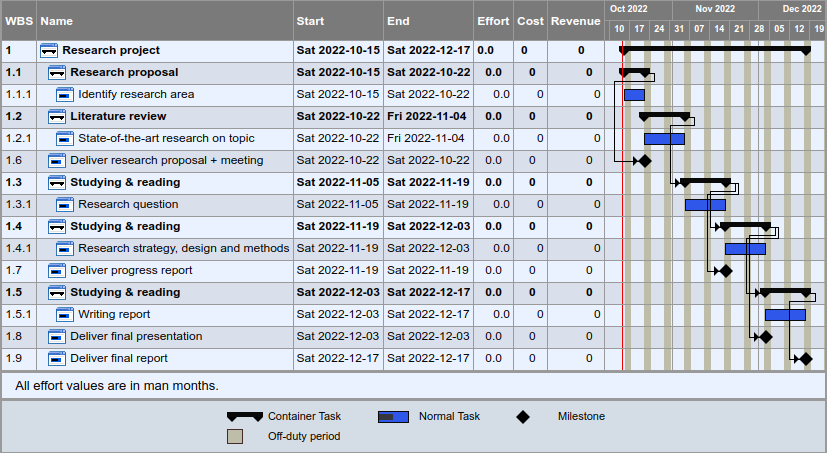
\includegraphics[width=.7\textwidth]{gantt.png}
      \end{figure}
\end{frame}

\appendix

\begin{frame}[allowframebreaks]
  \frametitle{参考文献}
  \printbibliography
\end{frame}

\makebottom

\end{document}
